% AI4BCI 2026: completed EEG study, revised 15 October 2026.
% Self-contained: official style, vector figure, and bibliography are embedded.
% Official workshop template verified 13 October 2026. Compile twice with pdflatex.
\begin{filecontents*}{ai4bci2026.sty}
\NeedsTeXFormat{LaTeX2e}
\ProvidesPackage{ai4bci2026}[2026/07/14 AI4BCI 2026 extended abstract style]

\RequirePackage[margin=0.75in]{geometry}
\RequirePackage{times}
\RequirePackage{microtype}
\RequirePackage{graphicx}
\RequirePackage{booktabs}
\RequirePackage{xcolor}
\RequirePackage{titlesec}
\RequirePackage{enumitem}
\RequirePackage{hyperref}

\definecolor{ai4bciblack}{HTML}{111111}
\definecolor{ai4bcigray}{HTML}{555555}

\hypersetup{
  colorlinks=true,
  linkcolor=ai4bciblack,
  citecolor=ai4bciblack,
  urlcolor=ai4bcigray
}

\setlength{\parindent}{0pt}
\setlength{\parskip}{4pt}
\setlength{\abovecaptionskip}{4pt}
\setlength{\belowcaptionskip}{0pt}
\setlist{nosep,leftmargin=*}

\titleformat{\section}
  {\large\bfseries}
  {\thesection}
  {0.6em}
  {}

\titleformat{\subsection}
  {\normalsize\bfseries}
  {\thesubsection}
  {0.6em}
  {}

\titlespacing*{\section}{0pt}{8pt}{3pt}
\titlespacing*{\subsection}{0pt}{6pt}{2pt}

\renewcommand{\maketitle}{
  \begin{center}
    {\LARGE\bfseries \@title \par}
    \vspace{0.55em}
    {\normalsize \@author \par}
  \end{center}
  \vspace{-0.5em}
}

\renewenvironment{abstract}
  {\section*{Abstract}\small}
  {\normalsize\vspace{0.2em}}

\pagestyle{plain}
\end{filecontents*}

\documentclass[11pt,a4paper]{article}
\usepackage{ai4bci2026}
\usepackage{amsmath,amssymb,pgfplots}
\usepackage[numbers,sort&compress]{natbib}
\pgfplotsset{compat=1.18}
\hypersetup{pdftitle={Recoverable Readout Mismatch in Smooth-to-Spiking EEG Decoding},
pdfauthor={Maximilian Nicholson}}

\title{Recoverable Readout Mismatch in\\Smooth-to-Spiking EEG Decoding}
\author{Maximilian Nicholson\\
University of Bath, United Kingdom\\
\texttt{mn866@bath.ac.uk}}
\date{}

\begin{document}
\maketitle

\begin{abstract}
Does near-chance performance after conversion reflect lost EEG information
or a failed readout? On BCI IV-2a (nine participants), we train and select on
session~1 and test on session~2. With the original architecture, converted heads yield
25.27--25.91\% balanced accuracy (BA); source-only
linear readouts on frozen spikes yield 38.69--42.37\%, without target labels
or encoder updates. Spiking probes trail smooth probes by 1.30--2.25
percentage points (pp). A post-study second encoder recovers 10.11 pp
[5.86, 14.29] through refitting. Sharpness-aware surrogate training (SAST)
\citep{nicholson,nicholsonOnSensor} does not demonstrate benefit over
compute-matched ordinary training ($-0.42$ pp, 95\% CI $[-2.88,2.67]$).
Source-only refitting diagnoses readout mismatch; equivalence and online
performance are not established.
\end{abstract}

\section{Methods}
\textbf{Data and separation.}
BCI Competition IV 2a has nine participants, four motor-imagery classes, and
22 EEG channels \citep{brunner}. Participant-specific models use session~1
runs~1--5 for training (240 trials), run~6 for validation (48), and all of
session~2 for testing (288). We retain artifact-marked trials, filter each
run at 4--38\,Hz, and extract 0--4\,s after the cue at 125\,Hz. Channel
normalization, checkpoint selection, and all main-analysis tuning use source
training/validation data only.

\textbf{Training and conversion.}
A temporal--spatial convolutional encoder has two leaky integrate-and-fire
blocks (16/32 channels, leak 0.9) and a time-averaged linear head. Smooth
training uses $\phi(v)=\tfrac12+\arctan(v)/\pi$ for threshold-centered $v$;
raw conversion uses $\mathbf{1}[v\geq0]$ with weights, threshold~1, and
previous-activity reset fixed. Ordinary training, its $2\times$-update control,
same-batch SAM \citep{foret}, and independent-batch SAST each have four
source-validation tuning candidates and five paired seeds. AdamW runs
800 updates (1,600 for the matched control); SAM/SAST use two gradient
evaluations per update. Direct hard-forward training shares the encoder;
EEGNet-8,2 \citep{lawhern} is a reference under the same 800-update budget. Calibration selects
one shared threshold from eight source-validation candidates over 0.25--3.
A post-study filter-bank common spatial pattern (FBCSP)-style reference
\citep{ang} uses nine bands within 4--38\,Hz, one-vs-rest spatial filters,
mutual-information feature selection, and shrinkage linear discriminant analysis;
four source-validation settings, one deterministic fit per participant.

\textbf{Readout diagnosis and inference.}
Matched ridge classifiers are fitted separately to smooth and spiking
final-layer features, using the same source-training labels and validation
penalty grid. Encoders remain frozen; no target labels enter fitting.
We report balanced accuracy (BA; chance 25\%), averaging seeds within
participants before 10,000 participant bootstrap resamples. Contrasts use
paired 95\% intervals. The primary contrast is calibrated SAST minus
matched ordinary training. Readout diagnostics were planned secondary
analyses; this study was not preregistered.
A post-study check repeats the readout analysis with a single-block depthwise LIF
encoder and four temporal bins (same nine participants, five seeds, source search).

\begin{figure}[!ht]
\centering
% BEGIN GENERATED READOUT PLOT
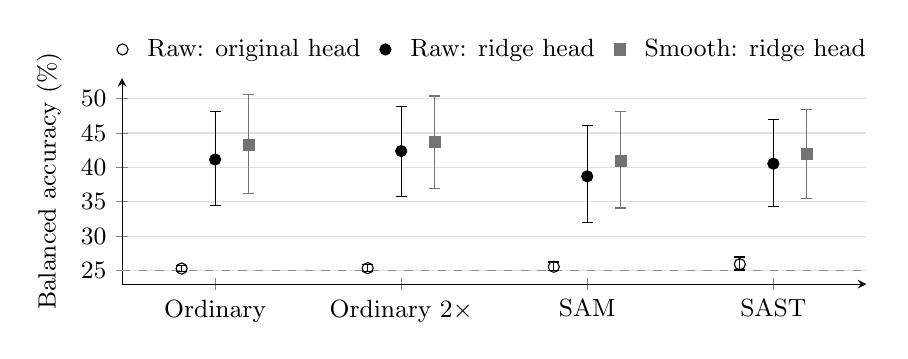
\begin{tikzpicture}
\begin{axis}[
width=0.91\linewidth,height=4.2cm,
xmin=-0.5,xmax=3.5,ymin=23,ymax=53,
xtick={0,1,2,3},xticklabels={Ordinary,Ordinary $2\times$,SAM,SAST},
ytick={25,30,35,40,45,50},ylabel={Balanced accuracy (\%)},
tick label style={font=\small},label style={font=\small},
axis lines=left,ymajorgrids,grid style={black!12},
legend style={font=\small,draw=none,at={(0.5,1.03)},anchor=south,column sep=5pt},
legend columns=3,legend cell align=left]
\addplot[black!45,dashed,forget plot] coordinates {(-0.5,25) (3.5,25)};
\addplot[only marks,black,mark=o,error bars/.cd,y dir=both,y explicit]
table[x=x,y=mean,y error minus=minus,y error plus=plus]{
x mean minus plus
-0.18 25.270061728 0.424382716 0.501543210
0.82 25.331790123 0.424382716 0.501543210
1.82 25.532407407 0.524691358 0.694444444
2.82 25.910493827 0.841049383 1.041666667
};
\addlegendentry{Raw: original head}
\addplot[only marks,black,mark=*,error bars/.cd,y dir=both,y explicit]
table[x=x,y=mean,y error minus=minus,y error plus=plus]{
x mean minus plus
0.00 41.134259259 6.658950617 7.044753086
1.00 42.368827160 6.620370370 6.536072531
2.00 38.688271605 6.774691358 7.338155864
3.00 40.532407407 6.288773148 6.412037037
};
\addlegendentry{Raw: ridge head}
\addplot[only marks,black!55,mark=square*,error bars/.cd,y dir=both,y explicit]
table[x=x,y=mean,y error minus=minus,y error plus=plus]{
x mean minus plus
0.18 43.225308642 7.083333333 7.400077160
1.18 43.665123457 6.728395062 6.712962963
2.18 40.933641975 6.844328704 7.206983025
3.18 41.905864198 6.419753086 6.520640432
};
\addlegendentry{Smooth: ridge head}
\end{axis}
\end{tikzpicture}
% END GENERATED READOUT PLOT
\caption{Source-only readout refitting recovers decoding across all four
training conditions. Points are nine-participant means; bars are 95\%
bootstrap intervals. The dashed line is chance. Both ridge heads use identical
source splits and tuning budgets; smooth original-head scores are in Table~\ref{tab:decoding}.}
\label{fig:readout}
\end{figure}

\section{Results}
\begin{table}[!ht]
\centering
\caption{Session~2 BA (\%), mean [95\% participant interval].
Calibration uses source labels only; -- indicates an inapplicable mode.}
\label{tab:decoding}
\small\setlength{\tabcolsep}{4pt}
\begin{tabular}{lccc}
\toprule
Decoder / training & Nonspiking & Raw spikes & Calibrated spikes \\
\midrule
% BEGIN GENERATED E1 ROWS
Ordinary & 41.2 [34.2, 48.8] & 25.3 [24.8, 25.8] & 32.7 [28.9, 36.8] \\
Ordinary, $2\times$ updates & 42.5 [35.4, 49.8] & 25.3 [24.9, 25.8] & 33.5 [30.2, 36.7] \\
Same-batch SAM & 37.6 [30.9, 44.8] & 25.5 [25.0, 26.2] & 32.3 [27.9, 37.2] \\
Independent SAST & 39.5 [33.2, 46.0] & 25.9 [25.1, 27.0] & 33.0 [29.1, 37.9] \\
Direct hard-forward & -- & 43.0 [35.9, 50.2] & 43.0 [35.9, 50.3] \\
EEGNet reference & 54.1 [43.8, 64.2] & -- & -- \\
% END GENERATED E1 ROWS
% BEGIN GENERATED FBCSP ROW
FBCSP-style reference & 61.8 [52.9, 70.1] & -- & -- \\
% END GENERATED FBCSP ROW
\bottomrule
\end{tabular}
\end{table}

\textbf{Conversion and the primary comparison.}
The original study's 270 main fits and 216 tuning fits completed. Raw conversion reduces mean
BA to near chance in every smooth-training condition (Table~\ref{tab:decoding}).
Source threshold calibration partly recovers accuracy. Calibrated SAST minus
matched ordinary training is $-0.42$ percentage points (pp), 95\% CI
$[-2.88,2.67]$; the artifact-free sensitivity gives $-0.32$ pp
$[-2.87,2.87]$. The interval spans zero and effects in both directions: the
study does not demonstrate SAST superiority or establish equivalence.

\textbf{Recovery with a frozen encoder.}
Source-fitted raw-spike probes reach 38.69--42.37\% BA
(Figure~\ref{fig:readout}). For SAST, refitting raises BA from 25.91\% to
40.53\%: $+14.62$ pp $[8.26,21.37]$. Refitting also helps smooth features
($+2.44$ pp $[1.33,3.51]$), so the entire raw-spike gain cannot be attributed
uniquely to conversion repair. Comparing matched probes, raw SAST remains
$1.37$ pp below smooth SAST (raw minus smooth: $[-2.03,-0.71]$); all four
methods retain a 1.30--2.25 pp deficit. Recovery coexists with residual loss
of linear decodability. The post-study FBCSP-style reference reaches 61.81\%
BA, exceeding EEGNet by $7.66$ pp $[3.67,11.91]$ on the same test split.

% BEGIN GENERATED ARCHITECTURE CHECK
\textbf{Post-study architecture check.} A second encoder yields 27.44\% raw BA and 37.55\% after source-only refitting (gain $+10.11$ pp $[5.86,14.29]$); recovery exceeds matched smooth refitting by $+7.09$ pp $[2.01,12.21]$.
% END GENERATED ARCHITECTURE CHECK

\section{Discussion}
For this offline task, frozen-readout failure overstates the loss of linearly
decodable EEG information. Before collecting target labels, refit matched smooth
and spiking readouts using source labels. Recovery does not demonstrate unchanged
neural computation or a causal effect of flatness.
Converted models remain below both EEGNet and the classical reference.
Nine participants, one dataset, and two LIF encoders limit generalization.
No online-control, clinical, or hardware-energy benefit is established.

\textbf{Data, code, and related work.}
This is secondary analysis of public EEG; no new participants were recruited.
Related work includes the author's SAST preprints \citep{nicholson,nicholsonOnSensor}
and a submitted, unpublished UniReps manuscript on representational fidelity.
The EEG evaluation and frozen-feature readout diagnosis are separate contributions.
Code and outputs: \url{https://github.com/PluvioXO/ai4bci2026-readout}.
% Author confirmation of any applicable secondary-analysis ethics approval or
% exemption is still required; no approval number or exemption is asserted.

\begin{thebibliography}{6}
\setlength{\itemsep}{0pt}
\setlength{\parskip}{0pt}
\bibitem{nicholson}
M.~Nicholson. \href{https://arxiv.org/abs/2603.18039}{Sharpness Aware Surrogate
Training for Spiking Neural Networks}. arXiv:2603.18039, 2026.

\bibitem{nicholsonOnSensor}
M.~Nicholson. \href{https://arxiv.org/abs/2604.09696}{Sharpness-Aware
Surrogate Training for On-Sensor Spiking Neural Networks}.
arXiv:2604.09696, 2026.

\bibitem{brunner}
C.~Brunner, R.~Leeb, G.~R.~M\"uller-Putz, A.~Schl\"ogl, and G.~Pfurtscheller.
\href{https://www.bbci.de/competition/iv/desc_2a.pdf}{BCI Competition 2008---Graz
data set A}. Dataset description, 2008.

\bibitem{foret}
P.~Foret, A.~Kleiner, H.~Mobahi, and B.~Neyshabur.
\href{https://arxiv.org/abs/2010.01412}{Sharpness-Aware Minimization for
Efficiently Improving Generalization}. ICLR, 2021.

\bibitem{lawhern}
V.~J.~Lawhern et~al.
\href{https://doi.org/10.1088/1741-2552/aace8c}{EEGNet: A compact convolutional
neural network for EEG-based brain--computer interfaces}.
J. Neural Eng., 15:056013, 2018.

\bibitem{ang}
K.~K.~Ang, Z.~Y.~Chin, C.~Wang, C.~Guan, and H.~Zhang.
\href{https://doi.org/10.3389/fnins.2012.00039}{Filter Bank Common Spatial Pattern
Algorithm on BCI Competition IV Datasets 2a and 2b}. Front. Neurosci., 6:39, 2012.
\end{thebibliography}

% The companion appendix is separate: the submission limit includes references.
% Do not concatenate it with this submission PDF unless the venue permits it.
\end{document}
